\documentclass[aps,prl,twocolumn,reprint,amsmath,amssymb]{revtex4-1}

\usepackage{epsfig,color,graphicx}
\begin{document}
\newcommand{\Ang}{\ensuremath{\mathring{\text{A}}}}
\newcommand{\ltwid}{\mathrel{\raise.3ex\hbox{$<$\kern-.75em\lower1ex\hbox{$\sim$}}}}
\newcommand{\gtwid}{\mathrel{\raise.3ex\hbox{$>$\kern-.75em\lower1ex\hbox{$\sim$}}}}
\newcommand{\ket}[1]{\ensuremath{\vert #1 \rangle}}
\newcommand{\bra}[1]{\ensuremath{\langle #1 \vert}}
\newcommand{\braket}[2]{\ensuremath{\langle #1 \vert #2 \rangle}} % bra-ket inner product
\newcommand{\ketbra}[2]{\ensuremath{\vert #1 \rangle \langle #2 \vert}} % ket-bra outer product
\newcommand{\op}[1]{\ensuremath{\hat{#1}}} % operator
%\newcommand{\sill}{\psi_\mathrm{SILL}}
\newcommand{\sill}{\psi}
\newcommand{\trace}{{\rm Tr}}
\newcommand{\ntilde}{\tilde{n}}
\newcommand{\stilde}{\tilde{s}}
\newcommand{\atilde}{\tilde{\alpha}}
\newcommand{\new}{\color{red}}
\newcommand{\old}{\color{black}}
\newcommand{\bea}{\begin{eqnarray}}
\newcommand{\eea}{\end{eqnarray}}
\newcommand{\br}{\ensuremath{\mathbf{r}}}
\def\nn{\nonumber\\}

\bibliographystyle{apsrev}

%\title{RZK: Robust linear-scaling optimization of nonorthogonal localized molecular orbitals in density functional theory}
\title{Solution to the problem of optimization of compact localized molecular orbitals in density functional theory}

\author{Yifei Shi}
%\affiliation{Department of Chemistry, McGill University, 801 Sherbrooke St. West, Montreal, QC H3A 0B8, Canada}
\author{Rustam Z. Khaliullin}
\email{rustam.khaliullin@mcgill.ca}
\affiliation{Department of Chemistry, McGill University, 801 Sherbrooke St. West, Montreal, QC H3A 0B8, Canada}

%\date{\today}

\begin{abstract}
%Despite being concept simplier and computationally advantageous to density-matrix DFT NON-orth MO LS DFT has not become 
Although density functional theory based on [strictly] localized nonorthogonal molecular orbitals is a conceptually simple and promising linear-scaling method [for nonmetallic systems] its development has been hindered because of the inherently difficult optimization of such orbitals. 
In this work, we identified the origin of the slow and unstable convergence and developed a robust linear-scaling optimization procedure with a low computational overhead. 
%In this work, we develop a new method that avoids the problem by modifying the preconditioned conjugate gradient method. The optimization directions causing the slow convergence is filtered out and neglected using the approximate Hessian. We show that, by removing these directions, the energy and other properties can be obtained accurately and the computational cost is significantly reduced. This corresponds to posing a relaxed orthogonality constrains on the molecuar orbits. 
We demonstrate the efficiency of the method on systems a variety of systems ranging from molecular liquids to semi-conductors and insulators [in static systems and ab initio molecular dynamics simulations]. 
% RZK0: greater detail in the abstract?
%Implications.  %Furthermore, although this method is not fully variational, it is still accurate enough to produce stable molecular dynamics in systems where chemical reactions happen.
\end{abstract}
\maketitle

%\emph{Introduction}

Kohn-Sham (KS) density functional theory (DFT) is currently the most popular electronic structure method. However, the computational cost of the conventional KS DFT grows cubically with the number of atoms preventing its application to large systems. To overcome this limitation, recent research has focused on the development of linearly scaling (LS) DFT methods~\cite{goedecker1999linear,bowler2012methods}. 
%RZK: perhaps it is worth mentioning that construction of the effective KS Hamiltonian is already linear, the current bottleneck is a cubically-scaling procedure for the optimization of electronic degrees of freedom.

%RZK: orbits -> orbitals
All LS DFT method utilize the localized nature of gapped systems. A large family of methods work with the one-electron density matrix (DM)\cite{li1993density,lee1996linear,li2003density,vandevondele2012linear}, $F(\mathbf{r},\mathbf{r}^{'})=\sum_i f_i \phi_i(\mathbf{r}) \phi_i(\mathbf{r}^{'})$, which decays exponentially in $|\mathbf{r}-\mathbf{r}^{'}|$.These include methods like the Fermi operator expansion~\cite{goedecker1994efficient,goedecker1995tight}, divide-and-conquer method~\cite{yang1991direct,yang1991local}, and density matrix minimization method\cite{li1993density}. However, in a typical electronic structure calculation, the number of atomic orbits (AOs) is much larger than the number of molecular orbits (MOs), thus DM methods generally need to handle larger matrices and more variational parameters, limiting the DM methods mostly to minimal-basis tight-binding problems. 

% RZK: AOs is only one type of localized basis set functions. Most LS codes do not use AOs. I would, therefore, replace "AOs" with "localized basis functions".
 
Another approach to LS DFT is based on local molecular orbits (LMO), where electrons can only occupy AOs of certain molecules. Since, generally speaking, locality and orthogonality are not simultaneously obtainable, non-orthogonal LMOs are generally used. 
% RZK: should we introduce NLMOs to designate nonorthogonal LMOs? 
To avoid the calculation of the inverse of MO overlap matrix, a series of work have focused on using new energy functionals~\cite{mauri1993orbital,kim1995total,ordejon1995linear}, or introducing extra optimization variables~\cite{burger2008linear,peng2013effective}. This approach has the advantage of using fewer variational parameters, being more intuitive, and providing additional useful information about charge transfer interactions~\cite{khaliullin2007unravelling,khaliullin2008analysis}. However, the LMO approach suffers from intrinsic convergence problems~\cite{ordejon1995linear,fattebert2004linear}.
%
%
%Furthermore it was also shown in \cite{ordejon1995linear} that the straightforward LMO calculation without using a new energy functional may end up in a set of MOs that are collapsing. And the new energy functionals may lead to multiple minima \cite{kim1995total}.
In addition to poor convergence, the optimization of (N)LMOs without imposed orthogonality constraints often leads to a state, in which LMOs becoming linearly dependent. Such an orbital collapse is illustrated by the value of the determinant of the MO overlap matrix in a straightforward energy minimization of a simple linear systems of four hydrogen fluoride molecules interacting through hydrogen bonds. We used DZVP basis set and preconditioned conjugate gradient algorithm. In Fig~\ref{fig:det} we show the determinant of the MO overlap matrix and the maximum norm of the energy gradient as a function of the minimization step. The minimization brings the state into a singular point and as a result the energy gradient does not vanish. This aggravates the convergence problem.

%RZK: it is important to state that electrons delocalize only to the neighbors, the problem does not happen in fully localized and fully delocalized case. To describe the system it is useful to use pictorial representation.

\begin{figure}
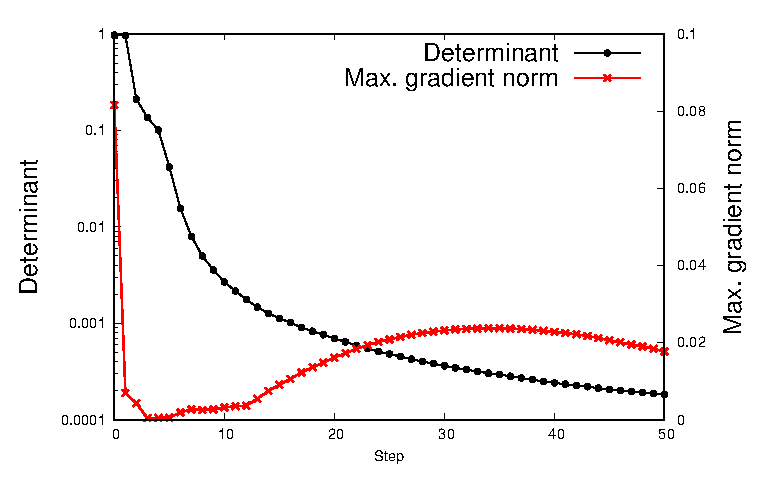
\includegraphics[width=0.5\textwidth]{det}
\caption{The determinant of the MO overlap matrix, and maximum norm of the energy gradient. }
\label{fig:det}
\end{figure}

Several efforts were made to deal with this problem. In~\cite{tsuchida2007augmented,tsuchida2008ab}, the MOs are forced to be orthogonal to an auxiliary wave function on a ``kernel region". Recently, in Ref.~\onlinecite{khaliullin2013efficient}, a block-diagonal reference is first calculated and then corretion which is constrained to be orthogonal to the reference is added in the second step. These two methods have all been successful in improving the convergence by constraining the MOs to be orthogonal to some reference states, thus requiring the reference to be somewhat physically meaningful. RZK: this only works for weakly-interacting molecular systems (the DOFs projected out already resemble the final occupied states)

Despite multiple potential advantages a reliable LMO-based LS method is still lacking for strongly interacting [nonmetallic] systems. In this work, we propose a new LS DFT method, based on LMOs, by identifying and filtering out the optimization directions that cause the slow convergence. We call it Hessian filter method and it has the advantage that: (a) The energy converges fast, and works with systems where interactions are strong. (b) No ``block-diagonal reference" or ``kernel region" are needed like in \cite{tsuchida2007augmented} or \cite{khaliullin2013efficient}.
%(b) The problem of orbital collapse is avoided. (c) Exact inverse of the MO overlap matrix is used, the inversion is linear when the overlap is sparse. This prevents the error introduced by approximate inverse overlap and the problem of multiple minima. 
(c) The problem of orbital collapse is avoided. (d) Although this method is not fully variational and the energy is not the minimum of any energy functional, it still produces stable dynamics for systems involving chemical reactions. 

%fragment -> center
\label{marker:theory} In the new LMO approach, all electrons are first logically assigned to \emph{localization centers}, each of which is represented by an atom [indices $x,y,z$]. A cutoff radius $R_c$ is then assigned to each center and its electrons are allowed to delocalize over basis functions of only neighbor centers within $R_c$. [indices $\bar{x}$] %Orbitals constructed in such a way represent electrons strictly localized in a spherical region of radius $R_c$ and are known as ALMOs, ELMOs, orbitals on compact support, nonorthogonal WFs, ZZZ. 
%
%They are expected to represent the maximally localized Wannier functions \cite{marzari1997maximally,he2001exponential}. 
%RZK: In addition to being spatially localized MLWFs satisfy other constraints, which are not imposed on LMOs. I would remove this comparison unless you think it is absolutely necessary.
%
While many previous works~\cite{ZZZ} dealt with weakly-interacting fragments (e.g. molecules) the new approach here represents the ultimate partitioning scheme.

% Matrices are bold %RZK0 define domain, define bars over fragment indices, spin-polarized case in the SI, Gamma-point, replace fragment with center.
In this work, fragments are denoted by $x,y,\ldots$, AOs are denoted by greek letters $\chi_\mu,\chi_\nu ..$, MOs are denoted by $\psi_i,\psi_j..$, $\chi_{x\mu}$ denotes the AOs which electrons in fragment $x$ can occupy. In this paper, the orbital indices are summed over but not fragment indices. Then MO $i$ in fragment $x$ can be expressed as:
\bea
\ket{\psi_{xi}} = \ket{\chi_{\bar{x}\mu}} {T^{\bar{x}\mu}}_{xi}
\label{eq:LMO}
\eea
%RZK: note the trick to keep up-down indices aligned

The AO to MO matrix $\mathbf{T}$ thus has blocked form, and the identity operator on fragment $x$ is:
%
\bea
\op{I}_{\bar{x}} = \ket{\chi_{\bar{x}\mu}} S^{\bar{x}\mu,\bar{x}\nu} \bra{ \chi_{\bar{x}\nu}}
\eea
%
where $S^{\bar{x}\mu,\bar{x}\nu}$ is the matrix element of the inverse overlap matrix $S_{\bar{x}\mu,\bar{x}\nu} = \braket{ \chi_{\bar{x}\mu}}{ \chi_{\bar{x}\nu}} $. In the case on LMOs, the KS DFT energy functional can be written in a conventional way but with the one-electron density matrix [operator] modified to take into account nonorthogonality of LMOs
\bea \label{eq:dm}
\op{R} = \sum_{x,y} \ket{\psi_{xi}} \sigma^{xi,yj} \bra{\psi_{yj}}
\eea
%
%RZK all matrices must be defined.

A straightforward minimization of the energy functional wrt $\mathbf{T}$ elements with a preconditioned conjugate gradient algorithm (PCG) has proven very reliable [low-prefactor method] for fully delocalized orbitals ($R_c \rightarrow \infty$) and completely localized orbitals ($R_c = 0$). PCG requires iterative evaluation of the energy gradient
%
\bea
{G_{\bar{x}\mu}}^{xi} \equiv \frac{\partial E}{\partial {T^{\bar{x}\mu}}_{xi}} = 4 \bra{\chi_{\bar{x}\mu}} (\op{I}-\op{R}) \op{H} \ket{\psi^{xi}}
\eea
%
and the [single] inversion of a local preconditioner defined on domain $\bar{x}$
%
\bea
P_{\bar{x}\mu,\bar{x}\nu} &=& s_{x} \bra{\chi_{\bar{x}\mu}} (\op{I}-\op{R}) \op{H}(\op{I}-\op{R}) + (\op{I}-\op{R}) \ket{\chi_{\bar{x}\nu}} 
\label{eq:hess}
\eea
%
This preconditioner is an easily-invertible approximation to the exact Hessian (the Supplementary Material and Ref.~\onlinecite{stoll1980use}) that was verified to provide the same rate/speed of convergence as the exact Hessian at a fraction of the inversion cost.
%
%where $S^x = P^x \cdot S \cdot P^x$ and $R^x = P^x \cdot R \cdot P^x$ are the projection of the overlap matrix and density matrix on fragment x. 
%
For [blocked-]LMOs, the PCG algorithm is/[could be] a very promising low-prefactor linear-scaling optimization algorithm because it replaces the cubically-scaling inversion with domain-by-domain inversion of very small locally-defined [SPD] matrices. Unfortunately, it as well as the Newton-Raphson algorithm based on the inversion of the exact Hessian suffers from the aforementioned slow convergence and orbital collapse problems. 
%
A closer inspection of the eigenvalues of the precoditioner obtained by solving the generalized eigenproblem on each domain 
%
\bea
%\mathbf{P}_{\bar{x}} \mathbf{A}_{\bar{x}} =  \mathbf{S}_{\bar{x}} \mathbf{A}_{\bar{x}} \Lambda_{\bar{x}} \\
P_{\bar{x}\mu,\bar{x}\nu} {A^{\bar{x}\nu}}_{xp} =  S_{\bar{x}\mu,\bar{x}\kappa} {A^{\bar{x}\kappa}}_{xp} \Lambda_{xp},
\label{eq:gev}
\eea
%
reveals the origin of this and other closely related previously reported problems. The eigenvalues, which represent the energy curvature in the optimization direction given by the corresponding eigenvector ${A^{\bar{x}\nu}}_{xp} \equiv \braket{\chi^{\bar{x}\nu}}{d_{xp}}$, can be divided into three categories according to their magnitude. The first (second) category includes zero (large) eigenvalues represent the optimization directions towards occupied (unoccupied) orbitals localized completely within the same domain. These two categories are the only ones present in the rapidly converging optimization of fully delocalized orbitals ($R_c \rightarrow \infty$) and completely localized orbitals ($R_c = 0$). The third category includes extremely small nonzero eigenvalues that appear when $R_c$ is finite and orbitals on different domains share basis set functions. 
An optimization along these shallow directions is extremely difficult because of unavoidable analytical approximations (e.g. approximate Hessian) and numerical noise (e.g. finite DFT grids) and thus represents the major barrier to the use of blocked-LMOs in LS DFT.

%, 

\label{marker:nature} What is the physical origin of the shallow optimization modes? It has been noted previously~\cite{goedecker1999linear} that one of the optimization problems of orbital-based LS DFT is due to the inexact invariance of the energy wrt the mixing of occupied orbitals. Although this is indeed the case for a series of approximate functionals proposed earlier~\onlinecite{Galli}, this problem is not present in the methods presented later~\cite{later} and described here because of the density matrix in Eq.~(\ref{eq:dm}) is constructed with the inverse of the overlap matrix and is properly idempotent [i.e. invariant to mixing among occupied states]. We instead suggest that the shallow directions correspond to the mixing with orbitals that are ``almost'' occupied. Indeed the number of shallow modes is typically equal to the number of occupied orbitals centered on the fragments with shared basis functions. This hypothesis is also supported by a comparison of the projector onto the shallow modes of $\bar{x}$
%
\bea
%W^{\bar{x}\mu,\bar{x}\nu} &=& {A^{\bar{x}\mu}}_{xp} \Theta_{xp} {A^{\bar{x}\nu}}_{xp} \\
\op{W}_{\bar{x}} &=& \ket{d_{xp}} \Theta_{xp} \bra{d_{xp}} 
\eea
%
with the projector of the occupied space onto $\bar{x}$
%
\bea
%C^{\bar{x}\mu,\bar{x}\nu} &\equiv& \bra{\chi^{\bar{x}\mu}} \op{C}_{\bar{x}} \ket{\chi^{\bar{x}\nu}} \\
\op{C}_{\bar{x}} &=& \sum_{y,z} \op{I}_{\bar{x}} \ket{\psi_{yi}} \sigma_{\bar{x}}^{yi,zj} \bra{\psi_{zj}} \op{I}_{\bar{x}}
\eea
%
In the former equation, $\Theta$ is a diagonal ``filter'' matrix whose diagonal elements are one if the eigenmode is considered shallow and zero otherwise. In the later equation, $\sigma_{\bar{x}}$ is the overlap matrix of $\bar{x}$-projected orbitals
\bea
\left(\sigma_{\bar{x}}\right)_{yi,zj} = \bra{\psi_{yi}} \op{I}_{\bar{x}} \ket{\psi_{zj}}
\eea

%The intuition from Eq~(\ref{eq:baddir}) implies that for each fragment $x$, each neighboring MO $|\psi_{yj}\rangle$ that only have a small portion outside of $x$ would contribute one problematic direction $P^x | \psi_{yj}\rangle$. And $Q^x$ should be a projector that removes all these directions, we assume MO $i$ on fragment $y$ that only have very small part outside of $x$, it will be denoted $xyi$, and the commen AOs of $x$ and $y$ fragments are denoted $xy\mu$, then $Q^x$ can be approximated as:
%%
%\bea
%(Q^x)^{x\mu,x\nu} \approx S^{x\mu,x\nu} - T^{xy\mu}_{yi} (\sigma^{-1})^{xyi,xzj} T^{xz\mu}_{zj}
%\label{eq:approxq}
%\eea

\label{marker:solution} As demonstrated below the two operators are almost exactly the same for a variety of systems. Thus the optimization along the shallow modes mixes orbitals that are almost completely but not quite occupied. Unsurprisingly, this often leads to collapse. In some extreme cases, there might be not sufficient DOFs within a domain to . We propose the following solution. Since [there is no sufficient DOFs to avoid bad modes] We propose to solve the problem by avoiding [the optimization along] these directions completely. [To this end,] We define a projector. So $Q^x$ is the operator the filters out the directions causes the slow optimization. We then define a new gradient and preconditioner that have correct tensorial properties:
%
\bea
%{G_{\bar{x}\mu}}^{xi} &=& ({\delta_{\bar{x}\mu}}^{\bar{x}\lambda} - S_{\bar{x}\mu,\bar{x}\nu} W^{\bar{x}\nu,\bar{x}\lambda}) {G_{\bar{x}\lambda}}^{xi} \nonumber \\
%
{Q_{\bar{x}\mu}}^{\bar{x}\lambda} &=& \bra{\chi_{\bar{x}\mu}} \op{I}_{\bar{x}} - \op{W}_{\bar{x}} \ket{\chi^{\bar{x}\lambda}} \\
\tilde{G}{_{\bar{x}\mu}}^{xi} &=& {Q_{\bar{x}\mu}}^{\bar{x}\lambda} {G_{\bar{x}\lambda}}^{xi} \\
%
\tilde{P}_{\bar{x}\mu,\bar{x}\nu} &=& {Q_{\bar{x}\mu}}^{\bar{x}\lambda} {P}_{\bar{x}\lambda,\bar{x}\gamma} {Q^{\bar{x}\gamma}}_{\bar{x}\nu}
\eea
%
The new gradient and preconditioner are used in the PCG algorithm. This new gradient is sensitive to occupied-occupied mixing, but neglects all small energy changes caused by the approximate invariance. This method resolves the convergence problem (see Fig ~\ref{fig:convergence} for a system of dimond silicon) while giving up a strict energy functional: the final energy may depend on the optimization path. However, we demenstrate that the energy is still accurate enough and can produce stable molecular dynamics nonetheless.
We also note that the preconditioner does not need to be calculated for each step, improving the efficiency of the optimization. 

We note that although $C$ and $W$ are very close, the more intuitive and easier-to-calculate $C$ cannot be used to eliminate the problematic directions completely and thus is not used to optimize LMOs.


\begin{figure}
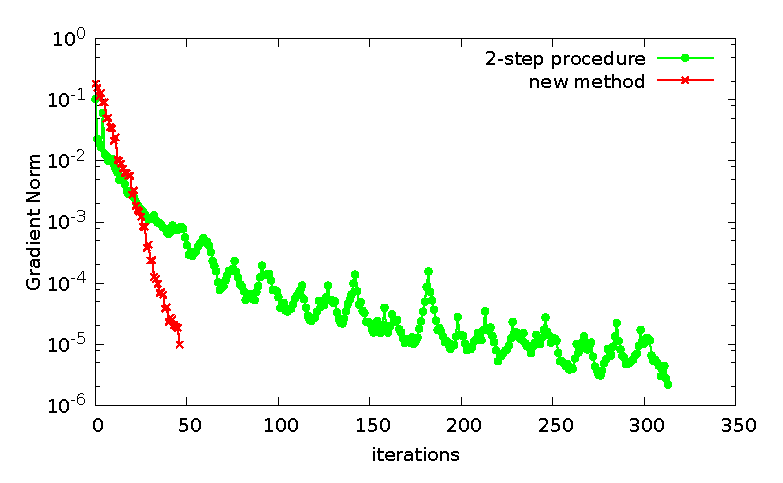
\includegraphics[width=0.5\textwidth]{convergence}
\caption{The maximun norm of energy gradient during the optimization. This is performed for 64 Si atoms with PBE exchange-correlation functional.}
\label{fig:convergence}
\end{figure}

\label{marker:results}
Our method is integrated with the CP2K package\cite{cp2kgeneral}, which uses the mixed Gaussian and plane wave method\cite{vandevondele2005quickstep}, and is an ideal platform for LS method. The optimization scheme is applied to systems with small band gap which are typically difficult for LS methods. The inversion of MO overlap matrix is carried out using Hotelling method \cite{hotelling1943some} which is linear scaling when the overlap matrix is sparse. Fig~\ref{fig:accuracy} shows the energy as a function of $R_c$ for several different systems: (a) CdSe of 768 atoms. (b) 64 water molecules, where each fragment is an atoms, and there are strong interaction and significant electron delocalization between fragments. (c) dimond Si of 512 atoms. We note that upon applying the filter $Q^x$ on the gradient, the final energy is no longer fully variational: the gradient is only zero in diretions that significantly change the energy. It also implies that the energy will depend on the optimization path. However, it is clear from Fig~\ref{fig:accuracy} that the energy converges to the DFT value as a function of cutoff, and the error mentioned is neglectable. 

\begin{figure}
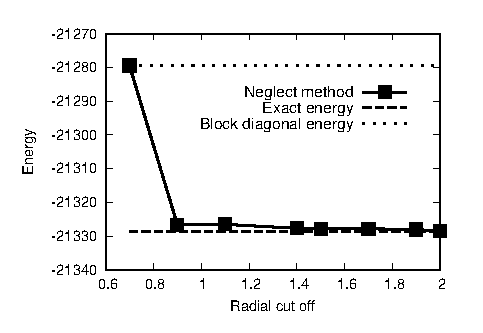
\includegraphics[width=0.35\textwidth]{CdSe}
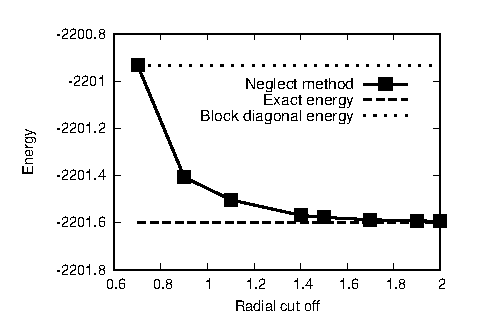
\includegraphics[width=0.35\textwidth]{H2O}
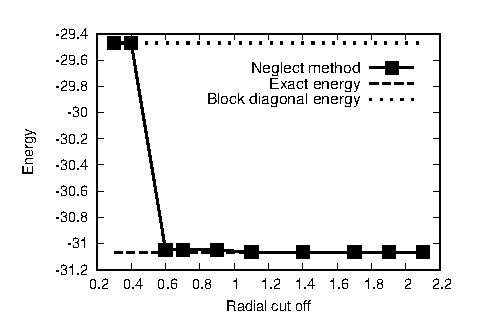
\includegraphics[width=0.35\textwidth]{Si}
\caption{The calculated energy as a function of the cutoff radii $R_c$. The systems involved are:(a) 128 water molecules with BLYP exchange-correlation functional and TZV2P basis set. Here each fragment is an atom, and covalent interactions happen between fragments. (b) 512 Silicon atoms with dimond lattice. PBE exchange-correlation functional and DZVP basis set are used. The convergence criteria used is $10^{-5}$.}
\label{fig:accuracy}
\end{figure}

\label{marker:performance}To test the linear efficiency of the method, we compare the calculation with orbital transformation (OT) \cite{weber2008direct,vandevondele2003efficient}, which is one of most optimized cubic scaling DFT method. The calculation is done for CdSe with different system sizes. The radial cutoff is set to be 0.9 vdWR, which from Fig~\ref{fig:accuracy} is enough to accurately describe the system. The result is shown in Fig~\ref{fig:scaling}. We note that our method is only linear scaling when the system is big enough so that the MO overlap matrix is sufficiently sparse, which for a dense system like CdSe takes many($\sim 3000$) atoms, resulting in the none-linear scaling behavior at small sizes.

\begin{figure}
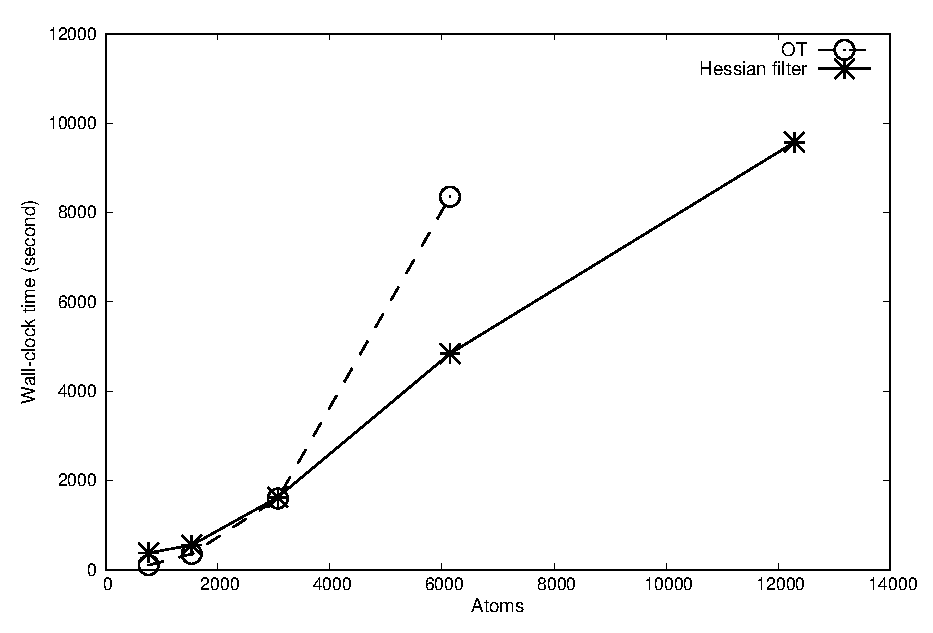
\includegraphics[width=0.45\textwidth]{timing}
\caption{Timing benchmark for the energy calculation of CdSe. The calculation is done on 256 cores. PBE exchange-correlation function is used and the radial cutoff is set to be 0.9 vDWR.}
\label{fig:scaling}
\end{figure}


\label{marker:moldyn}To further demonstrate the accuracy of the force and energy calculation, we run a molecular dynamics (MD) simulation on a system of 62 water molecules with 2 H$^+$ atoms. The 2 protons will hop around through OH covalent bond breaking and reforming. We show in Fig~\ref{fig:md} the conserved quantity and the potential energy in a MD run, proving that a stable simulation can be achieved with our method. We note that the Hellmann–Feynman theorem\cite{feynman1939forces} is used for the calculation of the force, this is in general only true when the energy is full variational, which is not true in our case. But the MD simulation further demonstrated that this error is neglectable, a conclusion already drawn from Fig~\ref{fig:accuracy}.

\begin{figure}
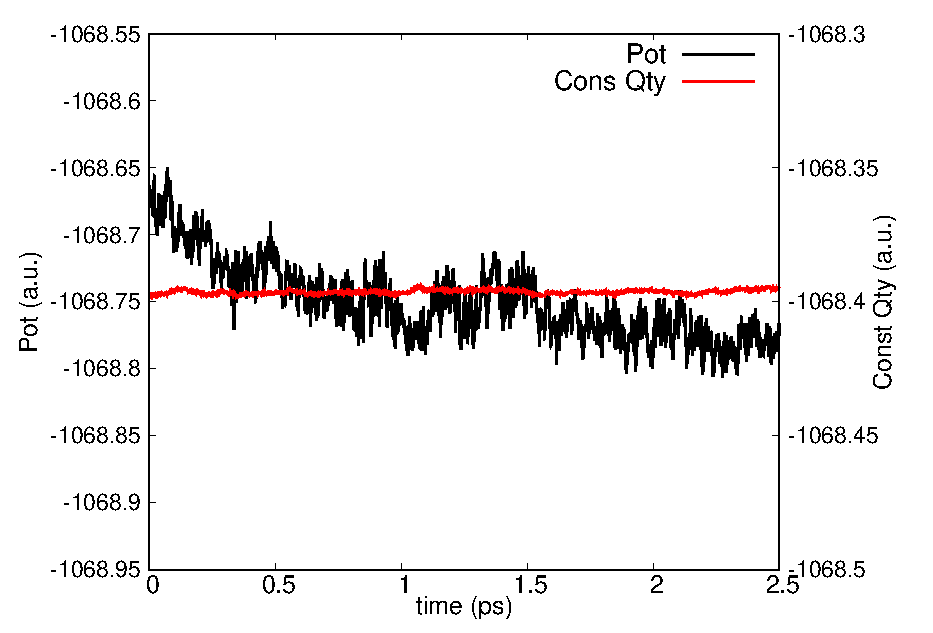
\includegraphics[width=0.45\textwidth]{const}
\caption{The total energy (kinetic plus potential) as a function of time, computed with linear scaling method and OT. Inset: the potential energy (Pot) and constant quantity (Const Qty) for linear scaling method.}
\label{fig:md}
\end{figure}


\label{marker:conclusion} We develop a new DFT method based on LMOs. The notorious convergence problem is avoided by identifying the small but none-zero eigenvalues of the Hessian. These directions are projected out from the gradient and the preconditioner, and the remaining gradient shows fast convergence with PCG. This projection can be understood as a relaxed orthogonality constrain for the LMOs. This method works even when the interaction and covalency between fragments are strong. We demonstrate the accuracy and efficiency of the method on systems like dimond silicon, CdSe. We also show a MD simulation in liquid water containing protons, and show that it can deal with systems where chemical reactions happen.

RZK To add: The physical meaning of Eq~\ref{eq:approxq} is a modified orthogonality constrain for LMOs. Orthognality and locality has generally been considered as competing properties: strict orthogonality leads to decaying tails, and for LMOs no orthogonality constrains are imposed except for MOs within a fragment. However, this causes the convergence problem previously mentioned: LMOs without orthogonality tends to collapse. Although global orthogonality cannot be achieved, we suggest a local orthogonality constrain, that the projection of MOs onto each fragment $x$ should be orthogonal. Unlike the case for none-local MOs, not every physical state can be transformed into such state.

\section{Acknowledgments} The research was funded by the Natural Sciences and Engineering Research Council of Canada through the Discovery Grant. The authors are grateful to Compute Canada and McGill HPC Centre for computer time.

\bibliography{negref}

\section{Supplemental Material}

Matrix equations clarify more compact operator expression used in the main text. 

The energy:
\bea
E[\{\psi_i\}] &=& 2\sum_{i,j} (\sigma^{-1})_{i,j}\int \psi_i(\br) (-\frac{1}{2}\nabla^2) \psi_j(\br)d\br \nonumber \\
&+& \frac{1}{2} \int \int \frac{\rho(\br)\rho(\br')}{|\br-\br'|}d\br d\br' + E_{XC}[\rho] \\
&+& 2\sum_{i,j} (\sigma^{-1})_{i,j}\int \psi_i(\br) V_{ext}({\br}) \psi_j(\br) d\br \nonumber
\eea

Contravariant density matrix:
%
\bea
\mathbf{R} = \mathbf{T} \sigma^{-1} \mathbf{T}^{\dagger}
\sigma = \mathbf{T}^{\dagger} \mathbf{S} \mathbf{T}
\eea
%
or, using the element by element notation,
%
\bea
R^{w\mu,z\nu} = \sum_{x,y}{T^{\overline{wx}\mu}}_{xi} \sigma^{xi,yj} {T^{\overline{zy}\nu}}_{yj}
\eea

The gradient for domain $\bar{x}$
%
\bea
\mathbf{G}_{\bar{x}x} = 4 \left[(\mathbf{I}-\mathbf{SR}) \mathbf{H} \mathbf{T}\sigma^{-1} \right]_{\bar{x}x}
\eea
%
or
%
\bea
{G_{\bar{x}\mu}}^{xi} = 4 \left[(\mathbf{I}-\mathbf{SR}) \mathbf{H} \mathbf{T}\sigma^{-1}\right]{_{\bar{x}\mu}}^{xi}
\eea
%

The preconditioner for domain $\bar{x}$
%
\bea
P_{\bar{x}\bar{x}} &=& s_x \left[(\mathbf{I}-\mathbf{SR}) \mathbf{H}(\mathbf{I}-\mathbf{RS}) + (\mathbf{I}-\mathbf{SRS})\right]_{\bar{x}\bar{x}} 
\eea 
%
\bea
P_{\bar{x}\mu,\bar{x}\nu} &=& s_x \left[(\mathbf{I}-\mathbf{SR}) \mathbf{H}(\mathbf{I}-\mathbf{RS}) + (\mathbf{I}-\mathbf{SRS})\right]_{\bar{x}\mu,\bar{x}\nu} 
\eea 

$\bar{x}$-coefficients of the $y$-centered orbitals projected onto $\bar{x}$-space are determined by
%
\bea
\op{I}_{\bar{x}} \ket{\psi_{yi}}  &=& \ket{\chi_{\bar{x}\mu}} S^{\bar{x}\mu,\bar{x}\nu} \braket{ \chi_{\bar{x}\nu}}{ \chi_{\bar{y}\lambda}}\, {T^{\bar{y}\lambda}}_{yi} = \nonumber \\
 &=& \ket{\chi_{\bar{x}\mu}} \left[ S^{\bar{x}\mu,\bar{x}\nu} S_{\bar{x}\nu,\bar{y}\lambda} {T^{\bar{y}\lambda}}_{yi} \right]
\eea 
%
Note that coefficients outside $\bar{x}$ may be nonzero but we do not need them.

\end{document}
